\documentclass[AMA,STIX1COL,]{WileyNJD-v2}


% For Pandoc highlighting needs

% Pandoc citation processing


\articletype{Research article}

\received{2022-05-09}

\revised{2022-05-09}

\accepted{2022-05-09}

\raggedbottom

\providecommand{\tightlist}{%
  \setlength{\itemsep}{0pt}\setlength{\parskip}{0pt}}

\begin{document}

\title{Interim sample size reestimation for adequately powered series of N-of-1 trials}

\author[a]{Daphne N. Weemering*}

\authormark{Weemering}

\address[a]{Department of Methodology and Statistics, Utrecht University, Utrecht, The Netherlands}

\corres{*D.N. Weemering, Padualaan 14, 3584 CH Utrecht. \email{d.n.weemering@students.uu.nl}}

\presentaddress{Padualaan 14, 3584 CH Utrecht, The Netherlands}

\abstract{Series of N-of-1 trials, i.e.~combined single patient multiple crossover randomized controlled trials (RCT), require a smaller sample size compared to standard RCT designs and can offer a solution in clinical research in populations of patients with rare diseases. In a priori sample size calculations, the specification of the nuisance parameters is often arbitrary and wrong, causing a greater risk of under- or overpowering a study. To overcome this problem, this thesis investigates the effectiveness and reliability of interim sample size reestimation based on nuisance parameter estimates in series of N-of-1 trials by means of simulation studies. Power, type I error rate and the sample size are important outcome measures. The results illustrate that interim sample size reestimation provides more adequately powered studies compared to the fixed sample size approach. Moreover, overall power is at the desired level of 0.80 or larger for most scenarios under the reestimation approach. The type I error rate appears to be somewhat inflated, which is likely caused by the small sample sizes. The median reestimated sample size shows to be close to the true sample size. Based on the results, the minimally required sample size for reliable reestimation could be established. Applying these requirements in practice could lead to better-powered series of N-of-1 trials.}

\keywords{N-of-1 trials; sample size reestimation; two-stage design; power; type I error; simulation study.}

\maketitle

\hypertarget{introduction}{%
\section{Introduction}\label{introduction}}

Randomized controlled trials (RCTs) are considered the gold standard in determining treatment efficacy in healthcare. At first glance, these standard RCTs seem to earn their position as the randomization of patients into a parallel experimental and control condition works quite well in balancing factors that are not under experimental control, allowing for unbiased estimation of the population treatment effect. A drawback, however, is that these standard RCTs require a relatively large sample size to establish the effectiveness of treatment with sufficient power. For the instances of finding the right intervention for patients with rare diseases, i.e., small patient populations, standard RCTs become therefore unfeasible.

The N-of-1 trial design can offer a solution for clinical research in small patient populations. A N-of-1 trial is a randomized controlled multiple crossover trial where a single patient repeatedly receives the experimental and control intervention in multiple cycles, where the allocation of the interventions in each cycle is in a random order \citep{guyatt1986}. As the experiment is conducted within a single patient, the advantage of the N-of-1 trial design is that a patient-specific treatment effect estimate is obtained. This allows these single patient trials to identify the best treatment for each patient \citep{kravitz2004}.

N-of-1 trials are suitable when the following requirements are met. First, the medical condition for which the intervention is prescribed should be chronic and (relatively) stable over time in order to reduce the chance that the progression of the disease can obscure the treatment differences between and within the trial cycles \citep{johnston2004, nikles2011}. Moreover, the intervention being tested in the N-of-1 trial should have a rapid on- and offset of biological action, and should have a short half-life to ensure that there is rapid washout as the cycles alternate \citep{nikles2011}. Additionally, the effect of the intervention should be measured using a validated (clinical) outcome measure. Choosing the right scale is necessary to ensure that the real clinical benefit is being measured. Lastly, the intervention used in the study should not alter the underlying condition, as this will make it unable to interpret the results for an individual as the trial progresses \citep{nikles2011}. This all necessitates careful selection of participants, short time cycles and relatively stable symptoms.

As results of a single N-of-1 trial are specific to an individual patient and can therefore not be generalized to the population, a single N-of-1 trial does not compare itself with a standard RCT. However, combining several individual N-of-1 trials, under the condition that the trials are similar, creates the possibility to estimate the population-level treatment effect \citep{zucker1997}. In the combined analysis of separate N-of-1 trials, now referred to a series of N-of-1 trials, both the magnitude of the average treatment effect as well as the heterogeneity in treatment response are taken into account \citep{zucker1997}. Comparing multiple treatment cycles combined with the recognition that the variability in response within individuals is usually lower than the variability between individuals, a smaller sample size is required to detect an effect of treatment in series of N-of-1 trials compared to parallel RCTs \citep{nikles2011}. This makes series of N-of-1 trials a valuable alternative to standard RCTs in the accumulation of a comprehensive evidence base in populations of people with rare diseases.

These series of N-of-1 trials have been performed for, among others, studying the effect of mexiletine on nondystrophic myotonia \citep{stunnenberg2018}, studying the effectiveness of methylphenidate on fatigue in patients with end-stage cancer \citep{mitchell2015}, and for investigating the usefulness of sildenafil on Raynaus-Phenomenon patients \citep{roustit2018}. Reasons for choosing the N-of-1 trial methodology vary, in general but also specifically for these aforementioned studies. The latter study chose to conduct a series of N-of-1 trials due to the heterogeneity in treatment response that should be taken into account, whereas the first two studies chose the N-of-1 trial methodology due to inability to achieve the required sample size for a standard RCT.

As in any clinical study, a priori sample size determination is necessary to avoid under- or overpowering the study, for planning on allocating resources and for assessing the feasibility of the study. Sample size formulas have been derived for series of N-of-1 trials for both random and fixed effects models \citep{senn2019}. As the main objective of combining the results of separate N-of-1 trials is to make inferences regarding the population treatment effect, random effects models are most appropriate and of interest here. For the sample size calculations, assumptions have to be made with regard to the parameters in the model, such as the clinically relevant difference and the nuisance parameters. However, the nuisance parameters in the model, which concern the within- and between subject variance of the response to treatment for series of N-of-1 trials \citep{araujo2016}, are generally unknown at the start of the study. Taking estimates of nuisance parameters from other studies can be unreliable because of differences in the study population, background conditions or study design \citep{zucker2002}. Furthermore, an estimate of the between subject variance in treatment response is often not available because the kind of study to obtain these estimates is a trial (or trials) incorporating such a component, such as a series of N-of-1 trials \citep{senn2016}. Series of N-of-1 trials are not (yet) that common, and even if similar series of N-of-1 trials exist, these kinds of estimates are usually not reported in the literature. Making unrealistic assumptions for these nuisance parameters can lead to substantial over- or underpowering, where the former exposes too many patients to potentially inferior treatment and the latter increases the risk of failing to identify a clinically relevant treatment effect due to a lack of power.

An appealing strategy for conquering the problem of incorrect assumptions for unknown nuisance parameters in sample size calculations is a two-stage design with interim sample size reestimation based on nuisance parameter estimates. With this design, the initially required sample size is calculated by making reasonable assumptions for the unknown nuisance parameters. Then, a portion of the data is collected up until a prespecified interim point along the trial and the unknown nuisance parameters are estimated using the data observed so far. These estimates are then used to update the power analysis and to adjust the sample size. Subsequently, the study is continued until the adjusted sample size is reached, and finally, the hypothesis is tested with all the data \citep{proschan2005}. Simulations studies have shown that this method has a high potential to protect from an incorrect sample size if the nuisance parameters were misspecified at the design stage of the study for standard RCTs \citep{wittes1990}. A distinction can be made between interim sample size reestimation based on nuisance parameter estimates and based on treatment effect estimates \citep{proschan2009}. This thesis will cover the first approach.

A concern with interim sample size reestimation based on estimates of nuisance parameters, is the inflation of the type I error rate \citep{kieser2000, wittes1990, birkett1994}. The method of interim sample size reestimation based on nuisance parameter estimates causes the total sample size to be dependent on the data that is obtained up until the interim point. A pooled estimate of the nuisance parameters, which is based on the combined data of the first and the second stage of the trial, is used for each nuisance parameter, which may cause the statistic to not be distributed as assumed in the final analysis under this approach. Therefore, the arguments leading to the assumed distribution may not be valid anymore \citep{kieser2000}. In this thesis it will be assessed whether the type I error rate becomes inflated for the proposed method considered here.

The application of interim sample size reestimation has not yet been investigated in the context of series of N-of-1 trials and no specific guidelines have been established. With this thesis, the usefulness and feasibility of interim sample size reestimation in series of N-of-1 trials will be investigated. With the use of simulation studies, the power of series of N-of-1 trials with interim sample size reestimation will be evaluated, and it will be compared with a similar design having a fixed sample size. Furthermore, the type I error rate for series of N-of-1 trials with interim sample size reestimation will be evaluated. Based on these results, the minimally required sample size for reliable interim sample size reestimation in series of N-of-1 trials will be determined.

The remainder of this thesis will be structured as follows: In section \ref{methods}, the notation, the model that is used for the simulation studies, sample size calculations and the analysis in series of N-of-1 trials are discussed. In section \ref{simulations} the design of the simulation studies in which power, the type I error rate and the reestimated sample size are evaluated will be explained. Section \ref{results} discusses the results of the simulations studies. And finally, this thesis is concluded with a discussion which is outlined in section \ref{discussion}.

\hypertarget{methods}{%
\section{Methodology}\label{methods}}

First, the methodology of a one-stage design for series of N-of-1 trials will be discussed in section \ref{onestage}. Here, the notation, the population model and sample size calculations for series of N-of-1 trials are introduced. In section \ref{twostage}, the procedure for interim sample size reestimation in series of N-of-1 trials will be outlined.

\hypertarget{onestage}{%
\subsection{One-stage design}\label{onestage}}

In a series of N-of-1 trials, each of the \(n\) subjects receives the experimental condition in one period and the control condition in the other period, each in \(k\) cycles of two periods. The order of treatment administration within each cycle will be randomly determined. At the end of each period, the outcome \(Y_{ijt}\) is measured, indicating the outcome for patient \(i\) (\(i = 1, ..., n\)) in cycle \(j\) (\(j = 1, ..., k\)) who is given treatment \(t\) (\(t = 1, 2\)). It is assumed that the disease under study is stable over time, that carryover effects are absent because of a sufficient duration of the washout period, and that there are no missing data. Furthermore, it is assumed that the outcome is a continuous measure and that it is normally distributed according to the following model:

\begin{equation} \label{eq:equation1}
Y_{ijt} = \lambda_i + \beta_{ij} + \epsilon_{ijt} + Z_{ijt}\tau_i
\end{equation}

In this model \citep{araujo2016}, \(\lambda_i \sim N(\Lambda, \phi^2)\) represents the random effect for subject \(i\), \(\beta_{ij} \sim N(0, \gamma^2)\) indicates the cycle effects for subject \(i\) in cycle \(j\), \(\epsilon_{ijt} \sim N(0, \sigma^2)\) represents the \(i\)-th subject's random error for the \(j\)-th cycle and treatment \(t\), and finally \(\tau_i \sim N(T, \psi^2)\) indicates the treatment effect for subject \(i\). \(Z_{ij1} = \frac{1}{2}\) and \(Z_{ij2} = -\frac{1}{2}\), indicating the received treatment for patient \(i\) in cycle \(j\). In this model, all the nuisance parameters are assumed to be independent of each other.

However, under the assumption that the data is complete, a simpler model for the treatment differences for subject \(i\) in cycle \(j\) can be derived from \eqref{eq:equation1} by subtracting for each cycle the subject's outcome observed under the control condition from the subject's outcome under the experimental condition. Then, \((Z_{ij1} - Z_{ij2})\) is equal to either \(1\) or \(-1\) depending on the random allocation of the experimental and control condition, and subsequently dividing by \((Z_{ij1} - Z_{ij2})\) will give the following model for the treatment differences \citep{araujo2016}:

\begin{equation} \label{eq:equation2}
d_{ij} = Y_{ij2} - Y_{ij1} = \tau_i + \zeta_{ij}
\end{equation}

Here, \(d_{ij}\) represents the observed treatment difference for patient \(i\) in cycle \(j\), where treatment 1 is consistently subtracted from treatment 2. \(\zeta_{ij} = \epsilon_{ij2} - \epsilon_{ij1}\), representing random within subject within-cycle disturbance terms. In this model, \(\tau_i \sim N(T, \psi^2)\), as before, and \(\zeta_{ij} \sim N(0, 2\sigma^2)\).

\hypertarget{sampcalc}{%
\subsubsection{Sample size calculations and analysis in N-of-1 trials}\label{sampcalc}}

From the model of the treatment differences in equation \eqref{eq:equation2}, the average treatment effect in the population and the corresponding variance can be derived, both necessary for calculating the required sample size. Following Senn \citep{senn2019}, an average treatment effect for each patient can be obtained:

\begin{equation} \label{eq:equation3}
\bar{d_{i.}} = \frac{\sum_{j=1}^{k} d_{ij}}{k}
\end{equation}

The average over all the \(n\) individual averages is equal to \(\hat{T} = \sum_{i=1}^{n} \sum_{j=1}^{k} d_{ij}/ nk\), which gives an estimate of the population treatment effect average and can be used to test the differences between the two treatments under investigation. The variance at the patient level, the variance of the \(n\) estimates of \(\bar{d_{i.}}\), then equals:

\begin{equation} \label{eq:equation4}
var(\bar{d_{i.}}) = \psi^2 + 2\sigma^2 /k
\end{equation}

The overall variance of the treatment estimate is then equal to \(var(\hat{T}) = \frac{\psi^2 + 2\sigma^2 / k}{n}\). The variance estimate at the patient level as shown in equation \eqref{eq:equation4} has \((n-1)\) degrees of freedom \citep{senn2019} and can be used to calculate the required sample size to achieve the desired power under hypothesized values for the nuisance parameters, \(\psi^2\) and \(\sigma^2\), now denoted as \(\psi^2_h\) and \(\sigma^2_h\), the clinically relevant difference \(\Delta\), and the two-sided significance level \(\alpha\) using a one sample \(t\)-test. For the calculation of the sample size, the standard deviation of the estimate in \eqref{eq:equation4} is used. The exact formula for the calculation of the sample size is based on a non-central \(t\)-distribution. Computation of the sample size therefore requires an iterative process and this can straightforwardly be done with the \texttt{pwr.t.test} function of the \texttt{pwr} package \citep{champely2018} in \texttt{R} \citep{Rmanual}.

\hypertarget{twostage}{%
\subsection{Two-stage design}\label{twostage}}

To cope with the problem around the a priori uncertainty regarding the nuisance parameters in the model, interim sample size reestimation is applied. For this process, the following steps are taken \citep{wittes1990, kieser2000, coffey1999}. First, the clinically relevant difference (\(\Delta\)), the type I error rate (\(\alpha\)), the desired power (\(1-\beta\)), the fraction of the initial sample size on which interim sample size reestimation will be based (\(f\)), the number of cycles (\(k\)) and the a priori hypothesized estimates for the nuisance parameters (\(\psi^2_h\) and \(\sigma^2_h\)) are specified. Then, \(\psi^2_h\) and \(\sigma^2_h\) are used to estimate the initial sample size \(n_0\) that yields the desired level of power. The sample size is calculated using \(var(\bar{d_{i.}})\) that is given in \eqref{eq:equation4}. All the estimated sample sizes are rounded up. After \(f*n_0 = n_{frac}\) patients are observed, the data that is collected is then used to estimate \(\hat{\sigma}^2\) and \(\hat{\psi}^2\), the estimates of the nuisance parameters at interim. These interim estimates should be used to find the new total sample size, \(n_1\), that is needed to achieve the target power. After the interim analysis the additional \(n_1 - n_{frac}\) patients should be observed. If the final sample size, \(n_1\) is larger than the already realized sample size \(n_{frac}\), the study is terminated and the final analysis is done. Otherwise, the additional data of \(n_1 - n_{frac}\) patients is collected and the final analysis is based on all the \(n_{frac} + (n_1-n_{frac})\) observations.

\hypertarget{simulations}{%
\section{Simulations}\label{simulations}}

Three simulation studies are performed to investigate the usefulness and reliability of interim sample size reestimation in series of N-of-1 trials. The first simulation study aims at evaluating the power and the expected sample size in series of N-of-1 trials that include interim sample size reestimation. The second simulation study aims at evaluating the power in series of N-of-1 trials under a fixed sample size approach. The results of the first and the second simulation study will be used to compare the power under the interim sample size reestimation approach in series of N-of-1 trials with the power under a fixed sample size approach. The third and final simulation study aims at evaluating the type I error rate of series of N-of-1 trials including interim sample size reestimation. When the effects of interim sample size reestimation in series of N-of-1 trials on the power and the type I error rate are established, the minimally required sample size that is necessary for reliable interim reestimation will be determined.

Various scenarios are considered for the simulation studies, each under different combinations of \(\psi_h^2\) and \(\sigma_h^2\), which are the hypothesized (a priori) values for the nuisance parameters that are used for the initial sample size calculation, \(f\), which represents the fraction of the initial sample size on which interim sample size reestimation will be based, and the actual values of the nuisance parameters which are used for generating the data, \(\psi_t^2\) and \(\sigma_t^2\). All the relevant parameters and parameter values considered in the simulation studies are displayed in table 1.

\begin{table}[h] 
\begin{center}
\caption{Parameters in the simulation studies.}
\begin{tabular}{p{8cm}p{6cm}} 
\hline
Description & Values \\
\hline 
\textbf{Design parameters} & \\
Fraction of initial sample size & $f = 0.25, 0.5, 0.75$ \\
Cycles per patient & $k = 3$ \\
Power & $1 - \beta = 0.8$ \\
Two-sided nominal significance level & $\alpha = 0.05$ \\
Clinically relevant difference & $\Delta = 1$ \\
\textbf{Model parameters} & \\
Within-patient within-cycle variance (data generation) & $\sigma^2_t = 0.25, 0.5, 1$ \\
Variance of treatment effect (data generation) & $\psi^2_t = 0.5, 1, 2$ \\
Within-patient within-cycle variance (hypothesized) & $\sigma^2_h = 0.25, 0.5, 1$ \\
Variance of treatment effect (hypothesized) & $\psi^2_h = 0.5, 1, 2$ \\
Average treatment effect & $T = 0, 1$  \\
\textbf{Simulation parameter} & \\
Number of simulation runs & $N = 10000$ \\
\hline 
\multicolumn{2}{l}{\textbf{Outcome parameters}} \\
Statistical power & Proportion of simulations runs in which the null hypothesis is correctly rejected when data is simulated under $T = 1$ \\
Type I error rate & Proportion of simulation runs in which the null hypothesis is falsely rejected when data is simulated under $T = 0$ \\
Sample size & Average and median sample size under reestimation for the $N$ simulation runs \\
\hline 
\end{tabular}
\end{center}
\end{table}

The simulation studies for the power and the type I error rate under interim sample size reestimation are performed following the procedure described in section \ref{twostage}. In the analysis, the null hypothesis that \(T=0\) will be tested against the alternative hypothesis that \(T=1\). First, the initial sample size \(n_0\) is calculated as the required sample size under \(T = 1\), \(k=3\), the type I error rate \(\alpha = 0.05\), the desired power \(1-\beta = 0.8\), \(\psi_h^2\) and \(\sigma_h^2\). The sample size calculations are performed using a two-tailed one sample \(t\)-test with the \texttt{pwr.t.test} function from the \texttt{pwr} package \citep{champely2018} in \texttt{R} (version 4.1.3) \citep{Rmanual}. Then, after calculating \(n_0\), a fraction of the initial sample size (\(n_0 * f\)) is calculated and data is generated for this fraction using the linear mixed model provided in equation \eqref{eq:equation2}. The data is generated under \(\psi_t^2\), \(\sigma_t^2\) and under \(T=1\) for the simulation study regarding the power. As \(\alpha\) is the probability of falsely rejecting the null hypothesis when it is true \citep{neyman1933}, the data will be generated under \(T = 0\) (and \(\psi_t^2\) and \(\sigma_t^2\)) for the simulation study regarding the type I error rate.

Based on the simulated data, a linear mixed model is fitted using the \texttt{lmer} function from the \texttt{lme4} package \citep{lme4} in \texttt{R} applying the model provided in equation \eqref{eq:equation2}. Restricted maximum likelihood (REML) will be applied to estimate the variance parameters, as this approach, to the contrary of ``regular'' maximum likelihood estimation (MLE), produces unbiased estimates for the variance components in the model for smaller sample sizes \citep{corbeil1976}. \(\hat{\psi}^2\) and \(\hat{\sigma}^2\), the interim estimates of the nuisance parameters, will be extracted and used to reestimate the sample size that is required under \(T = 1\), \(k = 3\), the type I error rate \(\alpha = 0.05\) and the desired power \(1-\beta = 0.8\). The \texttt{pwr.t.test} function is again utilized to calculate the sample sizes. For some scenarios, the standardized effect size (Cohen's \(d\)) becomes larger than 11 due to small values for \(\hat{\sigma}^2\) and \(\hat{\psi}^2\), resulting in a small sample size of approximately \(2\), which causes an error in the function. The standardized effect size is calculated as \(T/sd(\bar{d_{i.}})\), where \(sd(\bar{d_{i.}})\), as shown in section \ref{sampcalc}, is equal to \(\sqrt{\psi^2 + 2\sigma^2 /k}\). In those cases that Cohen's \(d \geq 11\), it will be set equal to \(10\). In all other cases, the calculated Cohen's \(d\) will be used for calculating the reestimated sample size \(n_1\). If \(n_1 \leq (n_0*f)\), no additional data is generated and the \(f*n_0\) data is used for the final analysis. If \(n_1 \geq (n_0*f)\), data is generated for the remaining sample size (\(n_1 - (f*n_0)\)).

For the final analysis, the linear mixed model provided in equation \eqref{eq:equation2} is fitted using the \texttt{lmer} function from the \texttt{lme4} package, and the \(p\)-value for the fixed effect is extracted. This process is iterated 10,000 times for each scenario (where each scenario regards a unique combination of \(\psi_t^2\), \(\sigma_t^2\), \(\psi_h^2\), \(\sigma_h^2\) and \(f\)). After all the simulation runs, power is calculated as the proportion of times in which the null hypothesis is correctly rejected when the data is simulated under \(T=1\). The type I error rate is then calculated as the proportion of times in which the null hypothesis is falsely rejected when the data is simulated under \(T=0\). Finally, the average sample size of the 10,000 simulation runs is calculated and the median reestimated sample size of the simulation runs is extracted.

The simulation study for the power under a fixed sample size approach is performed in a similar fashion as for the interim sample size reestimation approach, but of course excluding the process of reestimating the sample size. All other elements remain the same. The simulated data and the \texttt{R} code to obtain these data can be found in the \href{https://github.com/daphneweemering/MasterThesis}{Github repository} of this project.

\hypertarget{results}{%
\section{Results}\label{results}}

\hypertarget{power}{%
\subsection{Power}\label{power}}

First, the comparison of power under the interim sample size reestimation approach and the fixed sample size approach. Figure \ref{fig:fixedpower} displays the power for series of N-of-1 trials under the fixed sample size approach and figure \ref{fig:reestimpower} displays the power under the sample size reestimation approach (corresponding tables can be found in the appendix, tables A1 and A2 respectively). The power under the fixed sample size approach ranges from 0.32 to 1.00. Splitting up the power under the reestimation approach based on the fraction of the initial sample size that is used for reestimation, the range is {[}0.59; 0.89{]} when 25\% is used for reestimation, {[}0.73; 0.97{]} when 50\% is used, and {[}0.77; 1.00{]} when 75\% is used. Apparently, interim sample size reestimation is effective in the sense that the amount of underpowering is limited compared to the power under the fixed sample size approach. As can be seen in figures \ref{fig:fixedpower} and \ref{fig:reestimpower}, the power under the reestimation approach is under almost all scenarios closer to the desired level of 80\%.

The process of interim sample size reestimation appears to be able to make up for the misspecifications with regard to the nuisance parameters that were made during the design phase of series of N-of-1 trials, as overall power is higher when interim sample size reestimation is added to the design. Take for instance the scenario where \(\psi_t^2 = 0.5\) and \(\sigma_t^2 = 1\), and where \(\psi_h^2 = 0.5\) and \(\sigma_h^2 = 0.25\), quite a moderate scenario where \(\sigma^2\) is hypothesized to be lower than it is in the population. If one chooses to take the fixed sample size approach, the power of the study would be 60.8\%. However, taking the two-stage approach with interim sample size reestimation, the sample size is reconsidered somewhere along the trial, and the power is restored to 83.4\% when 75\% of the initial sample size is used to base reestimation on, 80.4\% when 50\% of the initial sample size is used, and 72.7\% when 25\% of the initial sample size is used for reestimation. Even though under some scenarios the power is still less than the desired level, overall it appears to be higher than it would have been under the fixed sample size approach.

\begin{figure}

{\centering 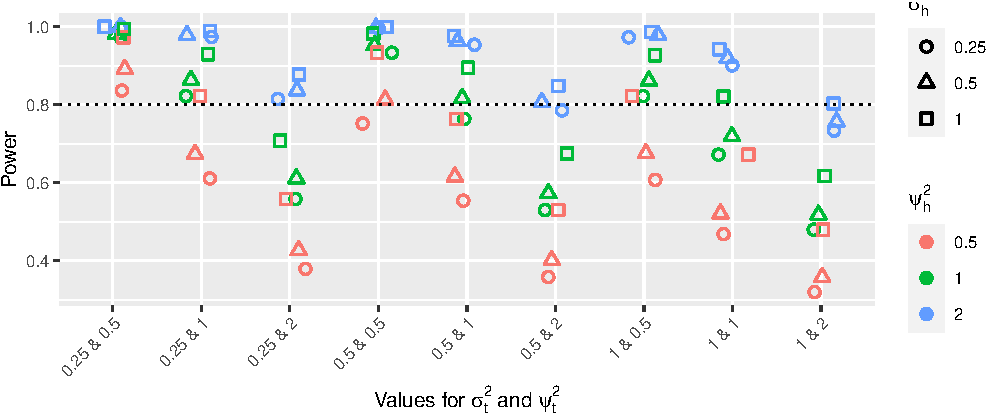
\includegraphics{Thesis_files/figure-latex/unnamed-chunk-2-1} 

}

\caption{Power in simulated series of N-of-1 trials with a fixed sample size under different data and hypothesized values for the nuisance parameters. The x-axis indicates the different combinations of the nuisance parameters for data generation $\sigma_t^2$ and $\psi_t^2$, respectively). The dotted line indicates a power of 0.8.\label{fig:fixedpower}}\label{fig:unnamed-chunk-2}
\end{figure}

Taking a closer look at the power of series of N-of-1 trials that include interim sample size reestimation, it appears that for most of the scenarios where \(f=0.5\) and \(f=0.75\), the power is approximately at the desired level of 80\% or higher. The scenarios where 50\% of the initial sample size is used for reestimation and where \(\psi_t^2 = 2\) and \(\psi_h^2 = 0.5\), and to a lesser extend also where \(\psi_t^2 = 2\) and \(\psi_h^2 = 1\), power below the desired level is still observed. However, this deficiency in power remains limited, the lowest power being 72.5\%. Overall, it appears that taking 50\% of the initial sample size to base reestimation on results in the highest chance of having an adequately powered series of N-of-1 trials. For those scenarios where \(f = 0.75\), power above the desired level of 80\% is not uncommon. Especially those scenarios where \(\psi_t^2 = 0.5\), the power often exceeds the desired level of 80\%. The fact that an excess of power is frequently observed when \(f = 0.75\) is probably due to a conservative sample size at the first stage of the trial. This causes the trial to be stopped at interim because too many subjects have already been observed.

\begin{figure}

{\centering 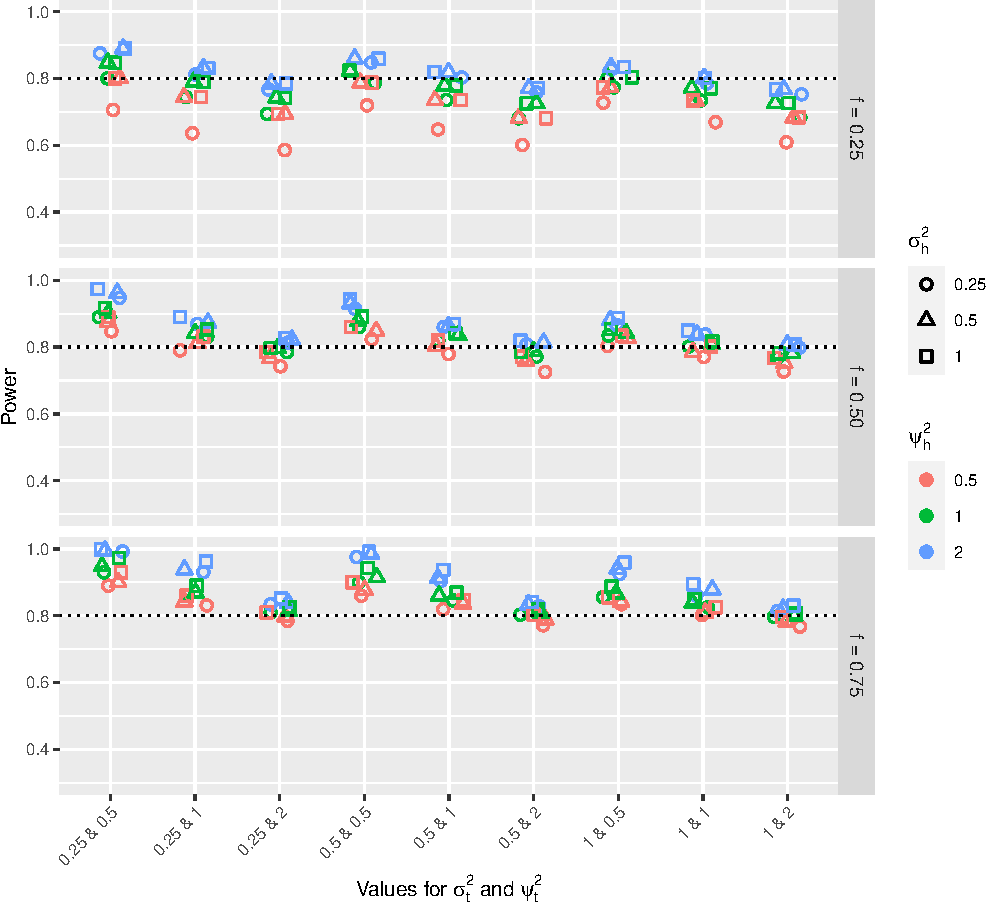
\includegraphics{Thesis_files/figure-latex/unnamed-chunk-4-1} 

}

\caption{Power in simulated series of N-of-1 trials with interim sample size reestimation under different data and hypothesized values for the nuisance parameters. The x-axis indicates the different combinations of the nuisance parameters for data generation ($\sigma_t^2$ and $\psi_t^2$, respectively). The dotted line indicates a power of 0.8.\label{fig:reestimpower}}\label{fig:unnamed-chunk-4}
\end{figure}

Power below the desired level is mostly observed for those scenarios where \(f=0.25\). Those scenarios where \(\psi_t^2 = 2\) and \(\psi_h^2 = 0.5\), regardless of the value of \(\sigma_h^2\), the power drops to even (approximately) 60\%. The scenarios where \(\psi_h^2 = 1\) lead to adequate power only where \(\psi_t^2\) is small. The scenarios where \(\psi_h^2 = 2\) result in adequately powered series of N-of-1 trials, with the exception of the scenarios where \(\psi_t^2 = 2\) (though, the power is not far off from the desired level of 80\% in these scenarios). Table 2 shows the sample sizes under the different values for \(\psi^2\) and \(\sigma^2\). The scenarios where the power is relatively low, there where \(\psi_h^2\) and \(\sigma_h^2\) are small, are the scenarios that base interim reestimation of the sample size on a very small initial sample size of 2 to 4 subjects.

\begin{table}[h] \label{table1}
\begin{center}
\caption{Sample sizes under $T = 1$, and various combinations of $\sigma^2$ and $\psi^2$.}
\begin{tabular}{l c c c c} 
\hline
$\sigma^2$ \& $\psi^2$ & Sample size & $f = 0.25$ & $f = 0.50$ & $f = 0.75$ \\
\hline 
$0.25$ \& $0.5$ & 7.38 (8) & 1.85 (2) & 3.69 (4) & 5.54 (6) \\
$0.25$ \& $1$ & 11.23 (12) & 2.81 (3) & 5.62 (6) & 8.42 (9) \\
$0.25$ \& $2$ & 19.02 (20) & 4.76 (5) & 9.51 (10) & 14.27 (15) \\
$0.5$ \& $0.5$ & 8.65 (9) & 2.16 (3) & 4.33 (5) & 6.49 (7) \\
$0.5$ \& $1$ & 12.52 (13) & 3.13 (4) & 6.26 (7) & 9.39 (10) \\
$0.5$ \& $2$ & 20.32 (21) & 5.09 (6) & 10.16 (11) & 15.24 (16) \\
$1$ \& $0.5$ & 11.23 (12) & 2.81 (3) & 5.62 (6) & 8.42 (9) \\
$1$ \& $1$ & 15.11 (16) & 3.78 (4) & 7.56 (8) & 11.33 (12) \\
$1$ \& $2$ & 22.93 (23) & 5.73 (6) & 11.47 (12) & 17.20 (18) \\
\hline 
\end{tabular}
\end{center}
\end{table}

\hypertarget{type-i-error}{%
\subsection{Type I error}\label{type-i-error}}

Figure \ref{fig:reestimalpha} shows the type I error rate under the various scenarios considered in this thesis (the corresponding table A3 can be found in the appendix). Where 25\% of the initially required sample size is used to base interim sample size reestimation on, the type I error rate appears to become inflated under all the scenarios that are considered. For some scenarios, such as the combination of \(\psi_t^2 = 0.25\), \(\sigma_t^2 = 0.5\), \(\psi_h^2 = 2\) and \(\sigma_h^2 = 1\), the inflation of the type I error rate remains limited. When 50\% of the initial sample size is used as a basis for interim reestimation of the sample size, the inflation of the type I error rate appears to be limited to a number of scenarios. Where \(\psi_h^2 = 2\), the largest value considered in this thesis, the type I error rate appears to be closest to the nominal \(\alpha\)-level of \(0.05\). The value of \(\psi_h^2\) seems to have the biggest impact on the type I error rate; the larger the value of \(\psi_h^2\), the smaller the inflation of the type I error rate.

When 75\% of the initial sample size is used for reestimation of the sample size at interim, it appears that the scenarios where \(\psi_h^2\) is hypothesized to be \(0.5\) result in an inflation of the type I error rate. The only scenario where this does not happen, is when \(\psi_t^2\) and \(\sigma_t^2\) are both small (\(0.5\) and \(0.25\) respectively). For most of the scenarios where \(\psi_h^2 = 2\), the type I error rate remains controlled. Where \(\psi_h^2 = 1\) it appears that the type I error rate also remains controlled for the scenarios where \(\psi_t^2 = 0.5\). The scenarios where \(\psi_t^2 = 2\) appear to lead to an inflated type I error rate. The inflation of the type I error rate remains limited, however, when \(\psi_h^2 = 2\).

From the results it becomes clear that the type I error rate is not stable and that its size is dependent on the scenario under consideration. Also, it appears that the value of \(\psi_h^2\) has a greater influence on the inflation of the type I error rate than the value of \(\sigma_h^2\). Especially those scenarios where small values for \(\psi^2\) are hypothesized, those scenarios where the initial sample size is relatively small, result in inflated type I error rates.

\begin{figure}

{\centering 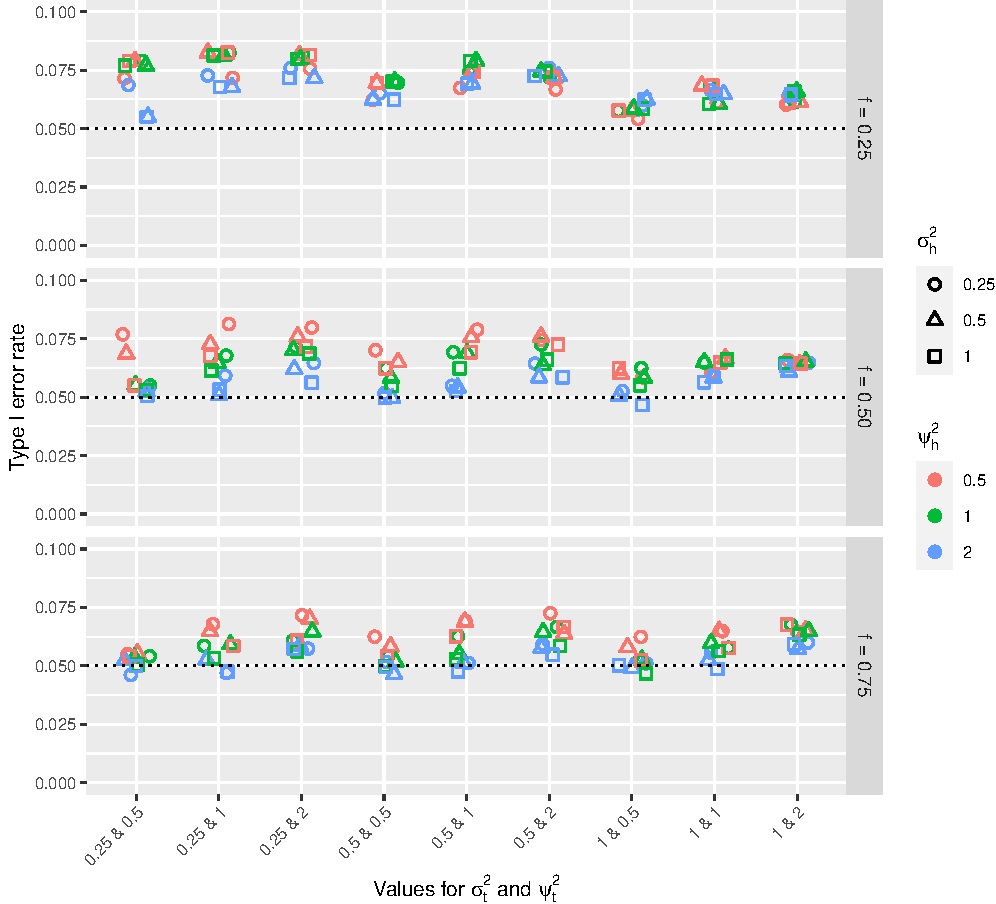
\includegraphics{Thesis_files/figure-latex/unnamed-chunk-6-1} 

}

\caption{Type I error rate in simulated series of N-of-1 trials under different data and hypothesized values for the nuisance parameters. The x-axis indicates the different combinations of the nuisance parameters for data generation ($\sigma_t^2$ and $\psi_t^2$, respectively). The dotted line indicates the nominal $\alpha$ level of 0.05. \label{fig:reestimalpha}}\label{fig:unnamed-chunk-6}
\end{figure}

\hypertarget{sample-size}{%
\subsection{Sample size}\label{sample-size}}

Finally, the evaluation of the results for the sample size. Figure \ref{fig:reestimsampsize} shows the median sample size and the minimum and maximum values for the sample size. These results can also be found in table A4 in the appendix. Table A5 in the appendix shows the average reestimated sample size and the corresponding standard deviation per scenario. First of all, it appears that for most scenarios the median reestimated sample size is close to the sample size under the true parameter values. Only those scenarios where the fraction of the initial sample size is fairly small, the reestimated sample size appears to be further away from the true sample size.

The values for \(\psi_h^2\) and \(\psi_t^2\) appear to have the greatest influence on the discrepancy between the median reestimated sample size and the true sample size. A large value for \(\psi_t^2\) combined with a small value for \(\psi_h^2\) appears to create the largest discrepancy between the median reestimated sample size and the true sample size. Scenarios where \(\psi_h^2 = 0.5\) also have a greater value for the maximum reestimated sample size, as can be seen in figure \ref{fig:reestimsampsize}. The standard deviation of the average reestimated sample size (table A5 in the appendix) is also relatively large for these scenarios. However, this variability is particularly high when 25\% of the initial sample size is used for reestimation, but reduces considerably when 50\% or 75\% of the initial sample size is used for reestimation. This all makes sense, as a larger sample size for reestimation allows for more reliable reestimation of the sample size, and hence, also less variability in reestimated sample sizes.

\begin{figure}

{\centering 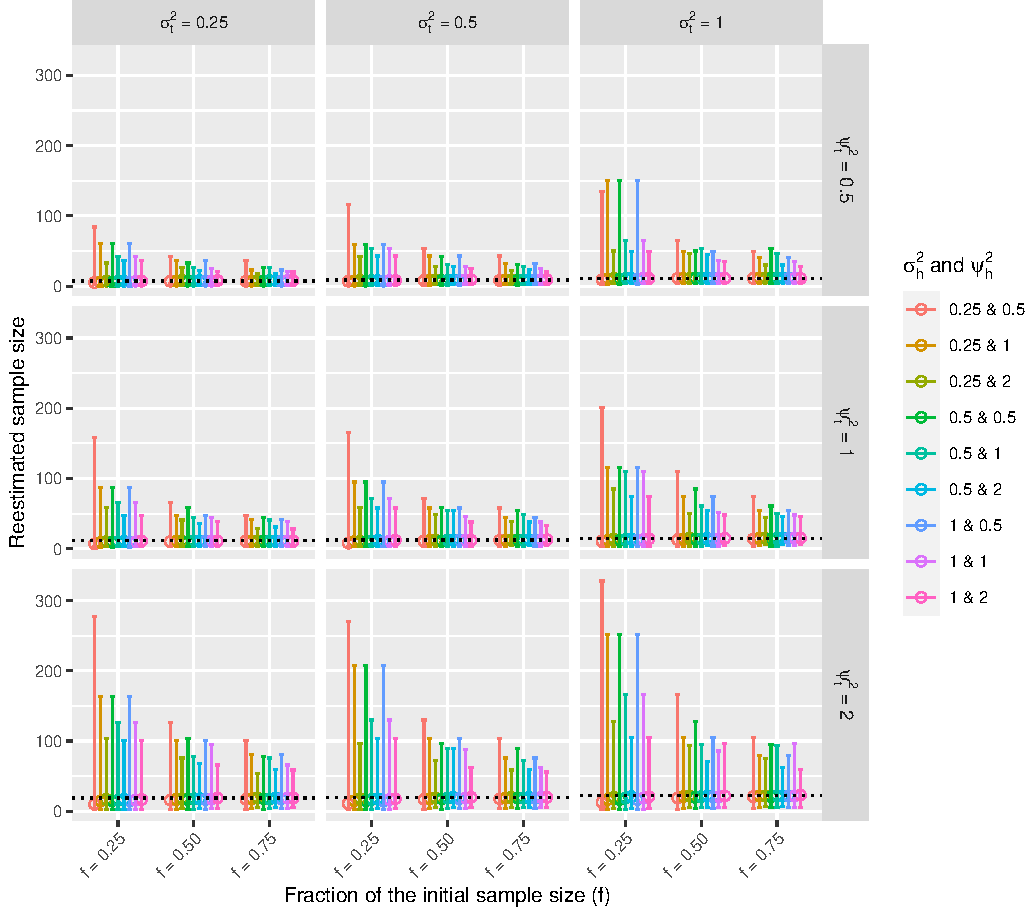
\includegraphics{Thesis_files/figure-latex/unnamed-chunk-8-1} 

}

\caption{Median (circles), minimum and maximum (error bars) reestimated sample sizes in simulated series of N-of-1 trials under different data, hypothesized values for the nuisance parameters, and fractions of the initial sample size. The dotted line indicates the sample size under the true values for the nuisance parameters.\label{fig:reestimsampsize}}\label{fig:unnamed-chunk-8}
\end{figure}

\hypertarget{discussion}{%
\section{Discussion}\label{discussion}}

The series of N-of-1 trials design offers a rigorous method for minimizing the sample size in clinical trials, offering opportunities for clinical research in populations of people with rare diseases, but also for general clinical research. The required sample size is determined by a number of factors, under which the population nuisance parameters which are, to the contrary of other factors such as the clinically relevant effect, generally unknown. There is usually considerable uncertainty about the values that are hypothesized for these unknown parameters. To deal with this problem, this thesis investigated the use of interim sample size reestimation in series of N-of-1 trials to contribute to the improvements of reliable trial methodology in populations of people with rare diseases. With interim sample size reestimation, the variances are estimated at an interim point during the clinical trials and those estimates are used to recalculate the sample size to make up for misspecifications prior to the trials.

In this thesis, three simulation studies are performed to examine the reliability of series of N-of-1 trials in terms of power and the type I error rate, and to compare series of N-of-1 trials including interim sample size reestimation with series of N-of-1 trials that have a fixed sample size. Based on the results for the power and type I error rate, recommendations will be made with regard to the minimally required sample size to base interim reestimation of the sample size on.

The results indicate that series of N-of-1 trials including interim sample size reestimation have power closer to the target power compared to series of N-of-1 trials with a fixed sample size. Especially for those trials where the misspecification of the nuisance parameters prior to the study was large compared to the population value, interim sample size reestimation in series of N-of-1 trials has a large positive impact on the power of the study in comparison with similar fixed sample size trials. When 50\% or 75\% of the initial sample size is used to base interim sample size reestimation on, almost all scenarios considered in this thesis will lead to a power of the desired 80\% or higher. For some scenarios, the power is larger than 80\%, and it could be argued that this is undesirable. However, due to the relatively small sample sizes under all the scenarios that are considered in this thesis, including one or two subjects too many will already lead to considerably higher power. Therefore, it could be argued that an excess of one or two patients is not so bad compared to an underpowered study where the results are not reliable. Incorporating interim sample size reestimation based on nuisance parameter estimates in the series of N-of-1 trials design can be a demonstrably improvement.

The type I error probabilities in series of N-of-1 trials appeared to be slightly inflated for some of the scenarios considered in this thesis. Small sample sizes can cause the estimation of the variance to be imprecise, which can lead to an inflated type I error rate. Wittes and colleagues \citep{wittes1999} have shown that for unrestricted interim sample size reestimation designs based on nuisance parameter estimates, where unrestricted indicates that the sample size could be both increased or decreased, the inflation of the type I error rate is especially present for small sample sizes. The inflation decreases when the sample size that is used for reestimation increases. This is in line with the results found in this thesis. Those scenarios where the initial sample size is larger appear to be quite closer to the nominal \(\alpha\)-level compared to the scenarios where a small sample size is considered. A sample size of 10 patients for the first stage of the trial appears to control the type I error rate quite well.

Considering that the type I error rate is more likely to be controlled at the nominal level when the initial sample size is relatively large, or at least large enough to estimate the nuisance parameters at interim more precisely, and that statistical power is also more adequate when a larger fraction of the initial sample size is used to base reestimation on, it appears to be best that the initial sample size is not too small. However, as this research focuses on improving trial designs for clinical research in small populations, it is also desirable to minimize the initial number of patients to include in a clinical study. So this is a trade-off. For adequately powered series of N-of-1 trials, the minimum fraction of the initial sample size for reliable interim sample size reestimation should be at least 6 patients. Table 2 shows the sample size for the different combinations of \(\psi^2\) and \(\sigma^2\), which gives an idea of which values lead to which sample sizes. For instance, the combination of \(\psi^2 = 1\), \(\sigma^2 = 0.25\) and \(f = 0.5\) will lead to an initial sample size of 6.

The type I error rate, however, might not always be controlled for when the fraction of the initial sample size for reestimation is equal to 6 patients. A fraction of the initial sample size of 12 patients keeps the type I error rate at approximately the nominal \(\alpha\)-level. Furthermore, methods to control the bias in the type I error rate at the nominal level exist \citep{proschan2005}, such as only using the second stage data for the final analysis \citep{stein1945}, or finding an adjusted \(\alpha\)-level for the test statistic \citep{kieser2000}. These methods, however, are not yet specified for the series of N-of-1 trials design. This can be an opportunity for future research.

A trade-off arises when a fraction of the initial sample size to base reestimation on should be chosen. The number of subjects in the first stage of the trial should not be to small, as this can have a negative impact on the power and the type I error rate, and thus on the reliability of the study. However, the number of subjects in the first stage should also not be too big, because this can cause reassessment to happen too late and can cause the sample size for 80\% power to have already been reached. Therefore, the recommendation is to use 75\% of the initial calculated sample size when it is relatively small (\(n_0 \leq 12\)), and to use 50\% of the initial calculated sample size otherwise. This way, the chances that the required final sample size has been exceeded before the interim reassessment of the sample size remain limited.

Some limitations of this study are acknowledged. First of all, only a limited number of design scenarios are discussed here. It was attempted to make the scenarios that are considered in this study as realistic as possible so that these are applicable to real life situations. However, other scenarios could lead to different results and implications. Second, practical issues such as carryover effects and selection bias, issues that can significantly influence the results, are not considered in the simulation studies of this thesis. Third, and last, this thesis does not investigate the effect of the relationship between the number of patients and the number of cycles within a patient on the sample size. Notice that the number of cycles only acts on one variance component of \(var(\hat{T})\) (see section \ref{sampcalc} for the formula), whereas increasing the number of subject acts on both variance components of \(var(\hat{T})\). Therefore, most gain is generally obtained by increasing the number of subjects. However, in cases where the number of subjects available is really limited and increasing the number of cycles appears to be more feasible, this would still be a useful addition to the literature of trial methodology.

\hypertarget{acknowledgements}{%
\section*{Acknowledgements}\label{acknowledgements}}
\addcontentsline{toc}{section}{Acknowledgements}

Ethical approval for this master thesis project was obtained from the Ethical Review Board of the Faculty of Social and Behavioural Sciences at Utrecht University (filed under number 21-1966).

\hypertarget{supporting-information}{%
\section*{Supporting information}\label{supporting-information}}
\addcontentsline{toc}{section}{Supporting information}

A complete research archive is available as a (public) \href{https://github.com/daphneweemering/MasterThesis}{Github repository} for this project, including the scripts for the simulation studies, the data, and the processing of the data.

\jnlcitation{\cname{%
\author{Weemering DN.}} \ctitle{Interim sample size reestimation for adequately powered series of N-of-1 trials}. \cjournal{Statistics in Medicine}. \cvol{2022;x(x):x--x}.}

\bibliography{bibfile.bib}


\newpage
\section{Appendix}

\begin{table}[ht]
\centering
\footnotesize
\renewcommand\thetable{A1}
\caption{Power of series of N-of-1 trials with a fixed sample size under different hypothesized and true values for the nuisance parameters.}
\makebox[\linewidth]{
\begin{tabular}{l c c c }
\toprule
 & $\psi_t^2 = 0.5; \sigma_t^2 = 0.25$ & $\psi_t^2= 1; \sigma_t^2= 0.25$ & $\psi_t^2 = 2; \sigma_t^2 = 0.25$ \\
\cline{2-4}
$\psi_h^2 = 0.5; \sigma_h^2 = 0.25$ & 0.836 & 0.611 & 0.379 \\
$\psi_h^2 = 1; \sigma_h^2 = 0.25$ & 0.973 & 0.822 & 0.558 \\
$\psi_h^2 = 2; \sigma_h^2 = 0.25$ & 0.999 & 0.974 & 0.815 \\
$\psi_h^2 = 0.5; \sigma_h^2 = 0.5$ & 0.892 & 0.674 & 0.427 \\
$\psi_h^2 = 1; \sigma_h^2 = 0.5$ & 0.981 & 0.864 & 0.611 \\
$\psi_h^2 = 2; \sigma_h^2 = 0.5$ & 1.000 & 0.979 & 0.837 \\
$\psi_h^2 = 0.5; \sigma_h^2 = 1$ & 0.973 & 0.822 & 0.558 \\
$\psi_h^2 = 1; \sigma_h^2 = 1$ & 0.994 & 0.930 & 0.708 \\
$\psi_h^2 = 2; \sigma_h^2 = 1$ & 1.000 & 0.989 & 0.878 \\
\hline 
& $\psi_t^2 = 0.5; \sigma_t^2 = 0.5$ & $\psi_t^2 = 1; \sigma_t^2 = 0.5$ & $\psi_t^2= 2; \sigma_t^2 = 0.5$ \\
\cline{2-4}
$\psi_h^2 = 0.5; \sigma_h^2 = 0.25$ & 0.752 & 0.554 & 0.358 \\
$\psi_h^2 = 1; \sigma_h^2 = 0.25$ & 0.933 & 0.764 & 0.530 \\
$\psi_h^2 = 2; \sigma_h^2 = 0.25$ & 0.995 & 0.954 & 0.786 \\
$\psi_h^2 = 0.5; \sigma_h^2 = 0.5$ & 0.813 & 0.615 & 0.401 \\
$\psi_h^2 = 1; \sigma_h^2 = 0.5$ & 0.952 & 0.817 & 0.573 \\
$\psi_h^2 = 2; \sigma_h^2 = 0.5$ & 0.997 & 0.963 & 0.807 \\
$\psi_h^2 = 0.5; \sigma_h^2 = 1$ & 0.933 & 0.764 & 0.530 \\
$\psi_h^2 = 1; \sigma_h^2 = 1$ & 0.983 & 0.895 & 0.675 \\
$\psi_h^2 = 2; \sigma_h^2 = 1$ & 0.999 & 0.976 & 0.849 \\
\hline 
& $\psi_t^2 = 0.5; \sigma_t^2 = 1$ & $\psi_t^2 = 1; \sigma_t^2 = 1$ & $\psi_t^2 = 2; \sigma_t^2 = 1$ \\
\cline{2-4}
$\psi_h^2 = 0.5; \sigma_h^2 = 0.25$ & 0.608 & 0.468 & 0.320 \\
$\psi_h^2 = 1; \sigma_h^2 = 0.25$ & 0.822 & 0.672 & 0.480 \\
$\psi_h^2 = 2; \sigma_h^2 = 0.25$ & 0.973 & 0.901 & 0.734 \\
$\psi_h^2 = 0.5; \sigma_h^2 = 0.5$ & 0.675 & 0.521 & 0.358 \\
$\psi_h^2 = 1; \sigma_h^2 = 0.5$ & 0.862 & 0.719 & 0.518 \\
$\psi_h^2 = 2; \sigma_h^2 = 0.5$ & 0.979 & 0.920 & 0.757 \\
$\psi_h^2 = 0.5; \sigma_h^2 = 1$ & 0.822 & 0.672 & 0.480 \\
$\psi_h^2 = 1; \sigma_h^2 = 1$ & 0.927 & 0.821 & 0.617 \\
$\psi_h^2 = 2; \sigma_h^2 = 1$ & 0.987 & 0.942 & 0.803 \\
\bottomrule
\end{tabular}}
\end{table}

\newpage
\begin{table}[ht]
\centering
\footnotesize
 \renewcommand\thetable{A2}
\caption{Power of series of N-of-1 trials including interim sample size reestimation under different hypothesized and true values for the nuisance parameters and under different fractions of the initial sample size.}
\makebox[\linewidth]{
\begin{tabular}{l c c c c c c c c c c c c}
\toprule
 & \multicolumn{3}{c}{$\psi_t^2 = 0.5; \sigma_t^2 = 0.25$} & \multicolumn{3}{c}{$\psi_t^2= 1; \sigma_t^2= 0.25$} & \multicolumn{3}{c}{$\psi_t^2 = 2; \sigma_t^2 = 0.25$} \\
\addlinespace[1pt]
\cmidrule(lr){2-4} \cmidrule(lr){5-7} \cmidrule(lr){8-10}
\textbf{\textit{f}} & \textbf{0.25} & \textbf{0.5} & \textbf{0.75} & \textbf{0.25} & \textbf{0.5} & \textbf{0.75} & \textbf{0.25} & \textbf{0.5} & \textbf{0.75} \\
\hline
$\psi_h^2 = 0.5; \sigma_h^2 = 0.25$ & 0.706 & 0.847 & 0.890 & 0.636 & 0.790 & 0.831 & 0.585 & 0.742 & 0.785 \\
$\psi_h^2 = 1; \sigma_h^2 = 0.25$ & 0.800 & 0.890 & 0.930 & 0.744 & 0.831 & 0.860 & 0.694 & 0.785 & 0.810 \\
$\psi_h^2 = 2; \sigma_h^2 = 0.25$ & 0.875 & 0.948 & 0.992 & 0.812 & 0.869 & 0.931 & 0.767 & 0.813 & 0.834 \\
$\psi_h^2 = 0.5; \sigma_h^2 = 0.5$ & 0.800 & 0.875 & 0.901 & 0.744 & 0.812 & 0.842 & 0.694 & 0.767 & 0.797 \\
$\psi_h^2 = 1; \sigma_h^2 = 0.5$ & 0.847 & 0.901 & 0.948 & 0.790 & 0.842 & 0.869 & 0.742 & 0.797 & 0.813 \\
$\psi_h^2 = 2; \sigma_h^2 = 0.5$ & 0.890 & 0.963 & 0.995 & 0.831 & 0.873 & 0.938 & 0.785 & 0.822 & 0.838 \\
$\psi_h^2 = 0.5; \sigma_h^2 = 1$ & 0.800 & 0.890 & 0.930 & 0.744 & 0.831 & 0.860 & 0.694 & 0.785 & 0.810 \\
$\psi_h^2 = 1; \sigma_h^2 = 1$ & 0.847 & 0.916 & 0.973 & 0.790 & 0.853 & 0.890 & 0.742 & 0.797 & 0.827 \\
$\psi_h^2 = 2; \sigma_h^2 = 1$ & 0.890 & 0.973 & 0.999 & 0.831 & 0.890 & 0.962 & 0.785 & 0.827 & 0.852 \\
\hline 
 & \multicolumn{3}{c}{$\psi_t^2 = 0.5; \sigma_t^2 = 0.5$} & \multicolumn{3}{c}{$\psi_t^2 = 1; \sigma_t^2 = 0.5$} & \multicolumn{3}{c}{$\psi_t^2= 2; \sigma_t^2 = 0.5$} \\
\addlinespace[1pt]
\cmidrule(lr){2-4} \cmidrule(lr){5-7} \cmidrule(lr){8-10}
\textbf{\textit{f}} & \textbf{0.25} & \textbf{0.5} & \textbf{0.75} & \textbf{0.25} & \textbf{0.5} & \textbf{0.75} & \textbf{0.25} & \textbf{0.5} & \textbf{0.75} \\
\hline
$\psi_h^2 = 0.5; \sigma_h^2 = 0.25$ & 0.720 & 0.823 & 0.860 & 0.647 & 0.779 & 0.819 & 0.601 & 0.725 & 0.771 \\
$\psi_h^2 = 1; \sigma_h^2 = 0.25$ & 0.787 & 0.860 & 0.900 & 0.735 & 0.819 & 0.846 & 0.681 & 0.771 & 0.803 \\
$\psi_h^2 = 2; \sigma_h^2 = 0.25$ & 0.848 & 0.915 & 0.976 & 0.803 & 0.860 & 0.904 & 0.758 & 0.808 & 0.829 \\
$\psi_h^2 = 0.5; \sigma_h^2 = 0.5$ & 0.787 & 0.848 & 0.877 & 0.735 & 0.803 & 0.835 & 0.681 & 0.758 & 0.788 \\
$\psi_h^2 = 1; \sigma_h^2 = 0.5$ & 0.823 & 0.877 & 0.915 & 0.779 & 0.835 & 0.860 & 0.725 & 0.788 & 0.808 \\
$\psi_h^2 = 2; \sigma_h^2 = 0.5$ & 0.860 & 0.930 & 0.984 & 0.819 & 0.862 & 0.912 & 0.771 & 0.813 & 0.833 \\
$\psi_h^2 = 0.5; \sigma_h^2 = 1$ & 0.787 & 0.860 & 0.900 & 0.735 & 0.819 & 0.846 & 0.681 & 0.771 & 0.803 \\
$\psi_h^2 = 1; \sigma_h^2 = 1$ & 0.823 & 0.891 & 0.942 & 0.779 & 0.842 & 0.869 & 0.725 & 0.785 & 0.819 \\
$\psi_h^2 = 2; \sigma_h^2 = 1$ & 0.860 & 0.942 & 0.992 & 0.819 & 0.869 & 0.937 & 0.771 & 0.819 & 0.841 \\
\hline 
 & \multicolumn{3}{c}{$\psi_t^2 = 0.5; \sigma_t^2 = 1$} & \multicolumn{3}{c}{$\psi_t^2 = 1; \sigma_t^2 = 1$} & \multicolumn{3}{c}{$\psi_t^2 = 2; \sigma_t^2 = 1$} \\
\addlinespace[1pt]
\cmidrule(lr){2-4} \cmidrule(lr){5-7} \cmidrule(lr){8-10}
\addlinespace[1pt]
\textbf{\textit{f}} & \textbf{0.25} & \textbf{0.5} & \textbf{0.75} & \textbf{0.25} & \textbf{0.5} & \textbf{0.75} & \textbf{0.25} & \textbf{0.5} & \textbf{0.75} \\
\hline
$\psi_h^2 = 0.5; \sigma_h^2 = 0.25$ & 0.727 & 0.804 & 0.834 & 0.669 & 0.771 & 0.802 & 0.609 & 0.727 & 0.767 \\
$\psi_h^2 = 1; \sigma_h^2 = 0.25$ & 0.773 & 0.834 & 0.855 & 0.734 & 0.802 & 0.825 & 0.683 & 0.767 & 0.797 \\
$\psi_h^2 = 2; \sigma_h^2 = 0.25$ & 0.827 & 0.866 & 0.925 & 0.785 & 0.838 & 0.860 & 0.753 & 0.798 & 0.815 \\
$\psi_h^2 = 0.5; \sigma_h^2 = 0.5$ & 0.773 & 0.827 & 0.842 & 0.734 & 0.785 & 0.809 & 0.683 & 0.753 & 0.782 \\
$\psi_h^2 = 1; \sigma_h^2 = 0.5$ & 0.804 & 0.842 & 0.866 & 0.771 & 0.809 & 0.838 & 0.727 & 0.782 & 0.798 \\
$\psi_h^2 = 2; \sigma_h^2 = 0.5$ & 0.834 & 0.880 & 0.940 & 0.802 & 0.838 & 0.878 & 0.767 & 0.808 & 0.820 \\
$\psi_h^2 = 0.5; \sigma_h^2 = 1$ & 0.773 & 0.834 & 0.855 & 0.734 & 0.802 & 0.825 & 0.683 & 0.767 & 0.797 \\
$\psi_h^2 = 1; \sigma_h^2 = 1$ & 0.804 & 0.854 & 0.887 & 0.771 & 0.817 & 0.849 & 0.727 & 0.782 & 0.808 \\
$\psi_h^2 = 2; \sigma_h^2 = 1$ & 0.834 & 0.887 & 0.959 & 0.802 & 0.849 & 0.894 & 0.767 & 0.808 & 0.830 \\
\bottomrule
\end{tabular}}
\end{table}


\newpage
\begin{table}[ht]
\centering
\footnotesize
 \renewcommand\thetable{A3}
\caption{Type I error rate of series of N-of-1 trials including interim sample size reestimation under different hypothesized and true values for the nuisance parameters and under different fractions of the initial sample size.}
\makebox[\linewidth]{
\begin{tabular}{l c c c c c c c c c c c c}
\toprule
 & \multicolumn{3}{c}{$\psi_t^2 = 0.5; \sigma_t^2 = 0.25$} & \multicolumn{3}{c}{$\psi_t^2= 1; \sigma_t^2= 0.25$} & \multicolumn{3}{c}{$\psi_t^2 = 2; \sigma_t^2 = 0.25$} \\
\addlinespace[1pt]
\cmidrule(lr){2-4} \cmidrule(lr){5-7} \cmidrule(lr){8-10}
\textbf{\textit{f}} & \textbf{0.25} & \textbf{0.5} & \textbf{0.75} & \textbf{0.25} & \textbf{0.5} & \textbf{0.75} & \textbf{0.25} & \textbf{0.5} & \textbf{0.75} \\
\hline
$\psi_h^2 = 0.5; \sigma_h^2 = 0.25$ & 0.071 & 0.077 & 0.055 & 0.072 & 0.081 & 0.068 & 0.076 & 0.080 & 0.072 \\
$\psi_h^2 = 1; \sigma_h^2 = 0.25$ & 0.079 & 0.055 & 0.054 & 0.083 & 0.068 & 0.059 & 0.082 & 0.072 & 0.061 \\
$\psi_h^2 = 2; \sigma_h^2 = 0.25$ & 0.069 & 0.053 & 0.046 & 0.073 & 0.059 & 0.047 & 0.076 & 0.065 & 0.057 \\
$\psi_h^2 = 0.5; \sigma_h^2 = 0.5$ & 0.079 & 0.069 & 0.055 & 0.083 & 0.073 & 0.065 & 0.082 & 0.076 & 0.070 \\
$\psi_h^2 = 1; \sigma_h^2 = 0.5$ & 0.077 & 0.055 & 0.053 & 0.081 & 0.065 & 0.059 & 0.080 & 0.070 & 0.065 \\
$\psi_h^2 = 2; \sigma_h^2 = 0.5$ & 0.055 & 0.052 & 0.052 & 0.068 & 0.051 & 0.053 & 0.072 & 0.062 & 0.059 \\
$\psi_h^2 = 0.5; \sigma_h^2 = 1$ & 0.079 & 0.055 & 0.054 & 0.083 & 0.068 & 0.059 & 0.082 & 0.072 & 0.061 \\
$\psi_h^2 = 1; \sigma_h^2 = 1$ & 0.077 & 0.053 & 0.051 & 0.081 & 0.061 & 0.053 & 0.080 & 0.069 & 0.056 \\
$\psi_h^2 = 2; \sigma_h^2 = 1$ & 0.055 & 0.051 & 0.050 & 0.068 & 0.053 & 0.048 & 0.072 & 0.056 & 0.057 \\
\hline 
 & \multicolumn{3}{c}{$\psi_t^2 = 0.5; \sigma_t^2 = 0.5$} & \multicolumn{3}{c}{$\psi_t^2 = 1; \sigma_t^2 = 0.5$} & \multicolumn{3}{c}{$\psi_t^2= 2; \sigma_t^2 = 0.5$} \\
\addlinespace[1pt]
\cmidrule(lr){2-4} \cmidrule(lr){5-7} \cmidrule(lr){8-10}
\textbf{\textit{f}} & \textbf{0.25} & \textbf{0.5} & \textbf{0.75} & \textbf{0.25} & \textbf{0.5} & \textbf{0.75} & \textbf{0.25} & \textbf{0.5} & \textbf{0.75} \\
\hline
$\psi_h^2 = 0.5; \sigma_h^2 = 0.25$ & 0.062 & 0.070 & 0.062 & 0.067 & 0.079 & 0.069 & 0.067 & 0.074 & 0.073 \\
$\psi_h^2 = 1; \sigma_h^2 = 0.25$ & 0.070 & 0.062 & 0.054 & 0.074 & 0.069 & 0.063 & 0.072 & 0.073 & 0.067 \\
$\psi_h^2 = 2; \sigma_h^2 = 0.25$ & 0.065 & 0.052 & 0.052 & 0.076 & 0.055 & 0.051 & 0.076 & 0.064 & 0.059 \\
$\psi_h^2 = 0.5; \sigma_h^2 = 0.5$ & 0.070 & 0.065 & 0.058 & 0.074 & 0.076 & 0.069 & 0.072 & 0.076 & 0.064 \\
$\psi_h^2 = 1; \sigma_h^2 = 0.5$ & 0.070 & 0.058 & 0.052 & 0.079 & 0.069 & 0.055 & 0.074 & 0.064 & 0.064 \\
$\psi_h^2 = 2; \sigma_h^2 = 0.5$ & 0.062 & 0.050 & 0.046 & 0.069 & 0.054 & 0.051 & 0.073 & 0.058 & 0.058 \\
$\psi_h^2 = 0.5; \sigma_h^2 = 1$ & 0.070 & 0.062 & 0.054 & 0.074 & 0.069 & 0.063 & 0.072 & 0.073 & 0.067 \\
$\psi_h^2 = 1; \sigma_h^2 = 1$ & 0.070 & 0.055 & 0.050 & 0.079 & 0.062 & 0.053 & 0.074 & 0.066 & 0.059 \\
$\psi_h^2 = 2; \sigma_h^2 = 1$ & 0.062 & 0.050 & 0.049 & 0.069 & 0.053 & 0.048 & 0.073 & 0.059 & 0.055 \\
\hline 
 & \multicolumn{3}{c}{$\psi_t^2 = 0.5; \sigma_t^2 = 1$} & \multicolumn{3}{c}{$\psi_t^2 = 1; \sigma_t^2 = 1$} & \multicolumn{3}{c}{$\psi_t^2 = 2; \sigma_t^2 = 1$} \\
\addlinespace[1pt]
\cmidrule(lr){2-4} \cmidrule(lr){5-7} \cmidrule(lr){8-10}
\textbf{\textit{f}} & \textbf{0.25} & \textbf{0.5} & \textbf{0.75} & \textbf{0.25} & \textbf{0.5} & \textbf{0.75} & \textbf{0.25} & \textbf{0.5} & \textbf{0.75} \\
\hline
$\psi_h^2 = 0.5; \sigma_h^2 = 0.25$ & 0.054 & 0.059 & 0.062 & 0.061 & 0.061 & 0.065 & 0.060 & 0.066 & 0.065 \\
$\psi_h^2 = 1; \sigma_h^2 = 0.25$ & 0.058 & 0.062 & 0.052 & 0.068 & 0.065 & 0.058 & 0.061 & 0.065 & 0.068 \\
$\psi_h^2 = 2; \sigma_h^2 = 0.25$ & 0.060 & 0.053 & 0.051 & 0.067 & 0.060 & 0.056 & 0.064 & 0.065 & 0.060 \\
$\psi_h^2 = 0.5; \sigma_h^2 = 0.5$ & 0.058 & 0.060 & 0.058 & 0.068 & 0.067 & 0.065 & 0.061 & 0.064 & 0.065 \\
$\psi_h^2 = 1; \sigma_h^2 = 0.5$ & 0.059 & 0.058 & 0.053 & 0.061 & 0.065 & 0.060 & 0.066 & 0.065 & 0.065 \\
$\psi_h^2 = 2; \sigma_h^2 = 0.5$ & 0.062 & 0.051 & 0.049 & 0.065 & 0.058 & 0.052 & 0.065 & 0.061 & 0.057 \\
$\psi_h^2 = 0.5; \sigma_h^2 = 1$ & 0.058 & 0.062 & 0.052 & 0.068 & 0.065 & 0.058 & 0.061 & 0.065 & 0.068 \\
$\psi_h^2 = 1; \sigma_h^2 = 1$ & 0.059 & 0.055 & 0.047 & 0.061 & 0.066 & 0.056 & 0.066 & 0.064 & 0.063 \\
$\psi_h^2 = 2; \sigma_h^2 = 1$ & 0.062 & 0.047 & 0.050 & 0.065 & 0.056 & 0.049 & 0.065 & 0.063 & 0.059 \\
\bottomrule
\end{tabular}}
\end{table}


\newpage
\begin{table}[ht]
\centering
\footnotesize
 \renewcommand\thetable{A4}
\caption{Median reestimated sample size [min;max in square brackets] in series of N-of-1 trials after interim sample size reestimation under different hypothesized and true values for the nuisance parameters and under different fractions of the initial sample size.}
\makebox[\linewidth]{
\begin{tabular}{l c c c c c c c c c}
\toprule
 & \multicolumn{3}{c}{$\psi_t^2 = 0.5; \sigma_t^2 = 0.25$} & \multicolumn{3}{c}{$\psi_t^2= 1; \sigma_t^2= 0.25$} & \multicolumn{3}{c}{$\psi_t^2 = 2; \sigma_t^2 = 0.25$} \\
\addlinespace[1pt]
\cmidrule(lr){2-4} \cmidrule(lr){5-7} \cmidrule(lr){8-10}
\textbf{\textit{f}} & \textbf{0.25} & \textbf{0.5} & \textbf{0.75} & \textbf{0.25} & \textbf{0.5} & \textbf{0.75} & \textbf{0.25} & \textbf{0.5} & \textbf{0.75} \\
\hline
\textbf{True sample size} & \multicolumn{3}{c}{\textbf{7.38}} & \multicolumn{3}{c}{\textbf{11.23}} & \multicolumn{3}{c}{\textbf{19.02}} \\
$\psi_h^2 = 0.5; \sigma_h^2 = 0.25$ & 5 [3;84] & 7 [3;42] & 7 [3;36] & 7 [3; 158] & 10 [3;66] & 11 [3;47] & 10 [3;277] & 16 [3;127] & 17 [3;101] \\
$\psi_h^2 = 1; \sigma_h^2 = 0.25$ & 6 [3;61] & 7 [3;36] & 7 [3;23] & 9 [3;87] & 11 [3; 47] & 11 [4;42] & 15 [3;164] & 17 [3;101] & 18 [4;81] \\
$\psi_h^2 = 2; \sigma_h^2 = 0.25$ & 7 [3;33] & 8 [3;26] & 8 [4;18] & 10 [3;59] & 11 [4;41] & 11 [4;29] & 17 [3;104] & 18 [4;76] & 19 [5;54] \\
$\psi_h^2 = 0.5; \sigma_h^2 = 0.5$ & 6 [3;61] & 7 [3;33] & 7 [3;27] & 9 [3;87] & 10 [3;59] & 11 [3;45] & 15 [3;164] & 17 [3;104] & 18 [3;78] \\
$\psi_h^2 = 1; \sigma_h^2 = 0.5$ & 7 [3;42] & 7 [3;27] & 8 [3;26] & 10 [3;66] & 11 [3;45] & 11 [4;41] & 16 [3;127] & 18 [3;78] & 18 [4;76] \\
$\psi_h^2 = 2; \sigma_h^2 = 0.5$ & 7 [3;36] & 8 [4;22] & 8 [4;18] & 11 [3;47] & 11 [4;36] & 11 [4;31] & 17 [3;101] & 18 [4;68] & 19 [5;60] \\
$\psi_h^2 = 0.5; \sigma_h^2 = 1$ & 6 [3;61] & 7 [3;36] & 7 [3;23] & 9 [3;87] & 11 [3;47] & 11 [4;42] & 15 [3;164] & 17 [3;101] & 18 [4;81] \\
$\psi_h^2 = 1; \sigma_h^2 = 1$ & 7 [3;42] & 7 [3;25] & 8 [4;21] & 10 [3;66] & 11 [3;45] & 11 [3;39] & 16 [3;127] & 18 [4;95] & 19 [4;66] \\
$\psi_h^2 = 2; \sigma_h^2 = 1$ & 7 [3;36] & 8 [4;21] & 8 [4;20] & 11 [3;47] & 11 [3;39] & 11 [4;28] & 17 [3;101] & 19 [4;66] & 19 [6;59] \\
\hline 
 & \multicolumn{3}{c}{$\psi_t^2 = 0.5; \sigma_t^2 = 0.5$} & \multicolumn{3}{c}{$\psi_t^2 = 1; \sigma_t^2 = 0.5$} & \multicolumn{3}{c}{$\psi_t^2= 2; \sigma_t^2 = 0.5$} \\
\addlinespace[1pt]
\cmidrule(lr){2-4} \cmidrule(lr){5-7} \cmidrule(lr){8-10}
\textbf{\textit{f}} & \textbf{0.25} & \textbf{0.5} & \textbf{0.75} & \textbf{0.25} & \textbf{0.5} & \textbf{0.75} & \textbf{0.25} & \textbf{0.5} & \textbf{0.75} \\
\hline
\textbf{True sample size} & \multicolumn{3}{c}{\textbf{8.65}} & \multicolumn{3}{c}{\textbf{12.52}} & \multicolumn{3}{c}{\textbf{20.32}} \\
$\psi_h^2 = 0.5; \sigma_h^2 = 0.25$ & 7 [3;116] & 8 [3;54] & 8 [3;43] & 8 [3;165] & 11 [3;72] & 12 [4;58] & 11 [3;270] & 17 [3;130] & 18 [4;104] \\
$\psi_h^2 = 1; \sigma_h^2 = 0.25$ & 7 [3;59] & 8 [3;43] & 9 [4;32] & 10 [3;95] & 12 [4;58] & 12 [4;44] & 15 [3;208] & 18 [4;104] & 19 [4;76] \\
$\psi_h^2 = 2; \sigma_h^2 = 0.25$ & 8 [3;42] & 9 [4;28] & 9 [4;22] & 11 [3;59] & 12 [4;49] & 12 [5;39] & 18 [3;97] & 19 [5;72] & 20 [6;59] \\
$\psi_h^2 = 0.5; \sigma_h^2 = 0.5$ & 7 [3;59] & 8 [3;42] & 8 [4;31] & 10 [3;95] & 11 [3;59] & 12 [4;54] & 15 [3;208] & 18 [3;97] & 19 [4;89] \\
$\psi_h^2 = 1; \sigma_h^2 = 0.5$ & 8 [3;54] & 8 [4;31] & 9 [4;28] & 11 [3;72] & 12 [4;54] & 12 [4;49] & 17 [3;130] & 19 [4;89] & 19 [5;72] \\
$\psi_h^2 = 2; \sigma_h^2 = 0.5$ & 8 [3;43] & 9 [4;28] & 9 [4;24] & 12 [4;58] & 12 [4;54] & 13 [5;38] & 18 [4;104] & 20 [5;89] & 20 [5;60] \\
$\psi_h^2 = 0.5; \sigma_h^2 = 1$ & 7 [3;59] & 8 [3;43] & 9 [4;32] & 10 [3;95] & 12 [4;58] & 12 [4;44] & 15 [3;208] & 18 [4;104] & 19 [4;76] \\
$\psi_h^2 = 1; \sigma_h^2 = 1$ & 8 [3;54] & 9 [3;28] & 9 [4;25] & 11 [3;72] & 12 [4;46] & 12 [4;38] & 17 [3;130] & 19 [4;88] & 20 [5;62] \\
$\psi_h^2 = 2; \sigma_h^2 = 1$ & 8 [3;43] & 9 [4;25] & 9 [4;20] & 12 [4;58] & 12 [4;38] & 13 [5;33] & 18 [4;104] & 20 [5;62] & 20 [6;56] \\
\hline 
 & \multicolumn{3}{c}{$\psi_t^2 = 0.5; \sigma_t^2 = 1$} & \multicolumn{3}{c}{$\psi_t^2 = 1; \sigma_t^2 = 1$} & \multicolumn{3}{c}{$\psi_t^2 = 2; \sigma_t^2 = 1$} \\
\addlinespace[1pt]
\cmidrule(lr){2-4} \cmidrule(lr){5-7} \cmidrule(lr){8-10}
\textbf{\textit{f}} & \textbf{0.25} & \textbf{0.5} & \textbf{0.75} & \textbf{0.25} & \textbf{0.5} & \textbf{0.75} & \textbf{0.25} & \textbf{0.5} & \textbf{0.75} \\
\hline
\textbf{True sample size} & \multicolumn{3}{c}{\textbf{11.23}} & \multicolumn{3}{c}{\textbf{15.11}} & \multicolumn{3}{c}{\textbf{22.93}} \\
$\psi_h^2 = 0.5; \sigma_h^2 = 0.25$ & 9 [3;135] & 11 [4;65] & 11 [4;49] & 11 [3;201] & 13 [4;110] & 14 [4;74] & 13 [3;328] & 19 [3;166] & 21 [4;105] \\
$\psi_h^2 = 1; \sigma_h^2 = 0.25$ & 10 [3;150] & 11 [4;49] & 11 [5;41] & 12 [3;116] & 14 [4;74] & 15 [5;54] & 17 [3;252] & 21 [4;105] & 22 [5;80] \\
$\psi_h^2 = 2; \sigma_h^2 = 0.25$ & 11 [4;50] & 11 [4;46] & 11 [6;30] & 14 [4;85] & 15 [4;50] & 15 [6;44] & 20 [4;128] & 22 [5;94] & 22 [7;75] \\
$\psi_h^2 = 0.5; \sigma_h^2 = 0.5$ & 10 [3;150] & 11 [4;50] & 11 [4;53] & 12 [3;116] & 14 [4;85] & 14 [4;61] & 17 [3;252] & 20 [4;128] & 21 [5;95] \\
$\psi_h^2 = 1; \sigma_h^2 = 0.5$ & 11 [4;65] & 11 [4;53] & 11 [4;46] & 13 [4;110] & 14 [4;61] & 15 [4;50] & 19 [3;166] & 21 [5;95] & 22 [5;94] \\
$\psi_h^2 = 2; \sigma_h^2 = 0.5$ & 11 [4;49] & 11 [4;45] & 11 [5;30] & 14 [4;74] & 15 [5;54] & 15 [6;46] & 21 [4;05] & 22 [5;71] & 22 [7;62] \\
$\psi_h^2 = 0.5; \sigma_h^2 = 1$ & 10 [3;150] & 11 [4;49] & 11 [5;41] & 12 [3;116] & 14 [4;74] & 15 [5;54] & 17 [3;252] & 21 [4;105] & 22 [5;80] \\
$\psi_h^2 = 1; \sigma_h^2 = 1$ & 11 [4;65] & 11 [4;37] & 11 [;35] & 13 [4;110] & 14 [4;52] & 15 [5;48] & 19 [3;166] & 21 [5;86] & 22 [6;97] \\
$\psi_h^2 = 2; \sigma_h^2 = 1$ & 11 [4;49] & 11 [5;35] & 11 [6;28] & 14 [4;74] & 15 [5;48] & 15 [6;46] & 21 [4;105] & 22 [6;97] & 23 [6;60] \\
\bottomrule
\end{tabular}}
\end{table}


\newpage
\begin{table}[ht]
\centering
\footnotesize
 \renewcommand\thetable{A5}
\caption{Average reestimated sample size (standard deviation in brackets) in series of N-of-1 trials after interim sample size reestimation under different hypothesized and true values for the nuisance parameters and under different fractions of the initial sample size.}
\makebox[\linewidth]{
\begin{tabular}{l c c c c c c c c c}
\toprule
 & \multicolumn{3}{c}{$\psi_t^2 = 0.5; \sigma_t^2 = 0.25$} & \multicolumn{3}{c}{$\psi_t^2= 1; \sigma_t^2= 0.25$} & \multicolumn{3}{c}{$\psi_t^2 = 2; \sigma_t^2 = 0.25$} \\
\addlinespace[1pt]
\cmidrule(lr){2-4} \cmidrule(lr){5-7} \cmidrule(lr){8-10}
\textbf{\textit{f}} & \textbf{0.25} & \textbf{0.5} & \textbf{0.75} & \textbf{0.25} & \textbf{0.5} & \textbf{0.75} & \textbf{0.25} & \textbf{0.5} & \textbf{0.75} \\
\hline
\textbf{True sample size} & \multicolumn{3}{c}{\textbf{7.38}} & \multicolumn{3}{c}{\textbf{11.23}} & \multicolumn{3}{c}{\textbf{19.02}} \\
$\psi_h^2 = 0.5; \sigma_h^2 = 0.25$ & 8.25 (7.20) & 7.94 (4.16) & 7.97 (3.25) & 12.11 (12.81) & 11.85 (7.15) & 11.79 (5.70) & 19.28 (23.26) & 19.69 (13.91) & 19.53 (10.73) \\
$\psi_h^2 = 1; \sigma_h^2 = 0.25$ & 8.12 (5.10) & 7.97 (3.25) & 7.90 (2.58) & 11.99 (9.17) & 11.79 (5.70) & 11.73 (4.54) & 19.69 (16.76) &  19.53 (10.73) & 19.45 (8.46) \\
$\psi_h^2 = 2; \sigma_h^2 = 0.25$ & 7.98 (3.64) & 7.88 (2.43) & 7.89 (1.93) & 11.74 (6.35) & 11.75 (4.33) & 11.76 (3.45) & 19.37 (11.70) &  19.49 (8.04) & 19.47 (6.36) \\
$\psi_h^2 = 0.5; \sigma_h^2 = 0.5$ & 8.12 (5.10) & 7.98 (3.64) & 7.95 (2.95) & 11.99 (9.17) & 11.74 (6.35) & 11.67 (5.22) & 19.69 (16.76) &  19.37 (11.70) & 19.60 (9.78) \\
$\psi_h^2 = 1; \sigma_h^2 = 0.5$ & 7.94 (4.16) & 7.95 (2.95) & 7.88 (2.43) & 11.85 (7.15) & 11.67 (5.22) & 11.75 (4.33) & 19.69 (13.91) & 19.60 (8.78) & 19.49 (8.04) \\
$\psi_h^2 = 2; \sigma_h^2 = 0.5$ & 7.97 (3.25) & 7.88 (2.31) & 7.87 (1.90) & 11.79 (5.70) & 11.78 (4.08) & 11.73 (3.31) & 19.53 (10.73) & 19.63 (7.58) & 19.42 (6.12) \\
$\psi_h^2 = 0.5; \sigma_h^2 = 1$ & 8.12 (5.10) & 7.97 (3.25) & 7.90 (2.58) & 11.90 (9.17) & 11.79 (5.70) & 11.73 (4.54) & 19.69 (16.76) & 19.53 (10.73) & 19.45 (8.46) \\
$\psi_h^2 = 1; \sigma_h^2 = 1$ & 7.94 (4.16) & 7.87 (2.71) & 7.85 (2.18) & 11.85 (7.15) & 11.84 (4.93) & 11.71 (3.84) & 19.69 (13.91) & 19.58 (9.08) & 19.63 (7.27) \\
$\psi_h^2 = 2; \sigma_h^2 = 1$ & 7.97 (3.25) & 7.85 (2.18) & 7.90 (1.79) & 11.79 (5.70) & 11.71 (3.84) & 11.75 (3.14) & 19.53 (10.73) & 19.63 (7.27) & 19.56 (5.84) \\
\hline 
 & \multicolumn{3}{c}{$\psi_t^2 = 0.5; \sigma_t^2 = 0.5$} & \multicolumn{3}{c}{$\psi_t^2 = 1; \sigma_t^2 = 0.5$} & \multicolumn{3}{c}{$\psi_t^2= 2; \sigma_t^2 = 0.5$} \\
\addlinespace[1pt]
\cmidrule(lr){2-4} \cmidrule(lr){5-7} \cmidrule(lr){8-10}
\textbf{\textit{f}} & \textbf{0.25} & \textbf{0.5} & \textbf{0.75} & \textbf{0.25} & \textbf{0.5} & \textbf{0.75} & \textbf{0.25} & \textbf{0.5} & \textbf{0.75} \\
\hline
\textbf{True sample size} & \multicolumn{3}{c}{\textbf{8.65}} & \multicolumn{3}{c}{\textbf{12.52}} & \multicolumn{3}{c}{\textbf{20.32}} \\
$\psi_h^2 = 0.5; \sigma_h^2 = 0.25$ & 10.07 (8.92) & 9.41 (5.02) & 9.33 (3.94) & 13.98 (14.88) & 13.18 (8.20) & 13.15 (6.44) & 22.22 (26.10) & 20.91 (14.67) & 20.72 (11.52) \\
$\psi_h^2 = 1; \sigma_h^2 = 0.25$ & 9.59 (6.16) & 9.33 (3.94) & 9.20 (3.16) & 13.49 (10.07) & 13.15 (6.44) & 13.02 (5.22) & 21.31 (18.53) & 20.72 (11.52) & 20.83 (9.12) \\
$\psi_h^2 = 2; \sigma_h^2 = 0.25$ & 9.40 (4.42) & 9.27 (2.99) & 9.15 (2.38) & 13.12 (7.13) & 13.03 (4.89) & 13.01 (3.97) & 21.09 (12.90) & 20.81 (8.53) & 20.83 (6.87) \\
$\psi_h^2 = 0.5; \sigma_h^2 = 0.5$ & 9.59 (6.16) & 9.40 (4.42) & 9.25 (3.54) & 13.49 (10.07) & 13.12 (7.13) & 13.06 (5.93) & 21.31 (18.53) & 21.09 (12.90) & 20..85 (10.30) \\
$\psi_h^2 = 1; \sigma_h^2 = 0.5$ & 9.41 (5.02) & 9.25 (3.54) & 9.27 (2.99) & 13.18 (8.20) & 13.06 (5.93) & 13.03 (4.89) & 20.91 (14.67) & 20.85 (10.30) & 20.81 (8.53) \\
$\psi_h^2 = 2; \sigma_h^2 = 0.5$ & 9.33 (3.94) & 9.17 (2.80) & 9.17 (2.36) & 13.15 (6.44) & 13.04 (4.61) & 13.06 (3.82) & 20.72 (11.52) & 20.73 (8.16) & 20.75 (6.65) \\
$\psi_h^2 = 0.5; \sigma_h^2 = 1$ & 9.59 (6.16) & 9.33 (3.94) & 9.20 (3.16) & 13.49 (10.07) & 13.15 (6.44) & 13.02 (5.22) & 21.31 (18.53) &  20.72 (11.52) & 20.83 (9.12) \\
$\psi_h^2 = 1; \sigma_h^2 = 1$ & 9.41 (5.02) & 9.28 (3.38) & 9.19 (2.71) & 13.18 (8.20) & 13.10 (5.50) & 13.00 (4.29) & 20.91 (14.67) & 20.81 (9.65) & 20.74 (7.70) \\
$\psi_h^2 = 2; \sigma_h^2 = 1$ & 9.33 (3.94) & 9.19 (2.71) & 9.14 (2.21) & 13.15 (6.44) & 13.00 (4.29) & 12.98 (3.52) & 20.72 (11.52) & 20.74 (7.70) & 20.90 (6.29) \\
\hline 
 & \multicolumn{3}{c}{$\psi_t^2 = 0.5; \sigma_t^2 = 1$} & \multicolumn{3}{c}{$\psi_t^2 = 1; \sigma_t^2 = 1$} & \multicolumn{3}{c}{$\psi_t^2 = 2; \sigma_t^2 = 1$} \\
\addlinespace[1pt]
\cmidrule(lr){2-4} \cmidrule(lr){5-7} \cmidrule(lr){8-10}
\textbf{\textit{f}} & \textbf{0.25} & \textbf{0.5} & \textbf{0.75} & \textbf{0.25} & \textbf{0.5} & \textbf{0.75} & \textbf{0.25} & \textbf{0.5} & \textbf{0.75} \\
\hline
\textbf{True sample size} & \multicolumn{3}{c}{\textbf{11.23}} & \multicolumn{3}{c}{\textbf{15.11}} & \multicolumn{3}{c}{\textbf{22.93}} \\
$\psi_h^2 = 0.5; \sigma_h^2 = 0.25$ & 13.70 (12.52) & 12.62 (6.89) & 12.23 (5.35) & 17.13 (17.44) & 16.32 (10.15) & 15.78 (7.96) & 24.59 (28.88) & 24.08 (17.00) & 23.57 (12.92) \\
$\psi_h^2 = 1; \sigma_h^2 = 0.25$ & 12.82 (8.43) & 12.23 (5.35) & 12.05 (4.26) & 16.54 (12.32) & 15.78 (7.96) & 15.73 (6.29) & 23.99 (20.32) & 23.57 (12.92) & 23.44 (10.33) \\
$\psi_h^2 = 2; \sigma_h^2 = 0.25$ & 12.37 (5.87) & 12.01 (4.07) & 11.86 (3.27) & 15.89 (8.74) & 15.73 (5.99) & 15.61 (4.91) & 23.71 (14.72) & 23.52 (9.76) & 23.37 (7.97) \\
$\psi_h^2 = 0.5; \sigma_h^2 = 0.5$ & 12.82 (8.43) & 12.37 (5.87) & 12.23 (4.99) & 16.54 (12.32) & 15.89 (8.74) & 15.73 (7.14) & 23.99 (20.32) & 23.71 (14.72) & 23.61 (11.94) \\
$\psi_h^2 = 1; \sigma_h^2 = 0.5$ & 12.62 (6.89) & 12.23 (4.99) & 12.01 (4.07) & 16.32 (10.15) & 15.73 (7.14) & 15.73 (5.99) & 24.08 (17.00) & 23.61 (11.94) & 23.52 (9.76) \\
$\psi_h^2 = 2; \sigma_h^2 = 0.5$ & 12.23 (5.35) & 11.92 (3.84) & 11.80 (3.16) & 15.78 (7.96) & 15.64 (5.70) & 15.65 (4.73) & 23.57 (12.92) & 23.44 (9.11) & 23.34 (7.64) \\
$\psi_h^2 = 0.5; \sigma_h^2 = 1$ & 12.82 (8.43) & 12.23 (5.35) & 12.05 (4.26) & 16.54 (12.32) & 15.78 (7.96) & 15.73 (6.29) & 23.99 (20.32) & 23.57 (12.92) & 23.44 (10.33) \\
$\psi_h^2 = 1; \sigma_h^2 = 1$ & 12.62 (6.89) & 12.08 (4.44) & 11.96 (3.71) & 16.32 (10.15) & 15.77 (6.66) & 15.65 (5.49) & 24.08 (17.00) & 23.43 (11.10) & 23.51 (8.95) \\
$\psi_h^2 = 2; \sigma_h^2 = 1$ & 12.23 (5.35) & 11.96 (3.71) & 11.85 (3.00) & 15.78 (7.96) & 15.65 (5.49) & 15.60 (4.43) & 23.57 (12.92) &  23.51 (8.95) & 23.53 (7.09) \\
\bottomrule
\end{tabular}}
\end{table}




\end{document}
